\chapter{Analysis techniques}

\intro{This chapter introduces the necessary toolset to perform the analyses within this thesis.}

%##############################################
\section{Event generation}
%##############################################

To compare reconstructed data with theoretical predictions, samples of simulated events are generated from theory and passed through a simulation of the \gls{cms} detector and emulation of its readout. The standard detector simulation is based on the Geant4 toolkit~\cite{Agostinelli2003250}. A fast alternative, the so-called ``FastSimulation'' package, exists within \gls{cms} as well~\cite{fsimRahmat}.

The event generation starts with the matrix element of a hard scattering process. \glshere{mc} methods are employed to sample the corresponding cross section integral. The advantage of \gls{mc}-based methods is that the variance of their result decreases as $1/n$ independently of the integral's dimensionality leading to an efficient convergence compared to quadrature-based methods~(e.g. Simpson's rule, Newton-Cotes). A commonly used \gls{mc} method is the \gls{vegas} algorithm~\cite{OHL199913} which is based on importance sampling where the integral is sampled not uniformly but along an adaptive importance function instead. The resulting sample of events reflects the probability distribution of a process over its phase space. Typically a reweighting is performed in addition such that all events contribute the same probability (e.i. they carry the same absolute weight). 

After obtaining events from the hard interaction, a \glshere{ps} program simulates the hadronization of final state partons. In addition, the radiation of gluons or quarks from initial or final state partons is accounted for as well as contributions from the underlying event including secondary low-$\pt$ interactions and color reconnection effects. A sketch of the various parts within an exemplary event is shown in Fig.~\ref{fig:technique-mcevent}. The \gls{ps} simulation is based on Altarelli-Parisi splitting functions~\cite{Altarelli:1977zs} which allow to calculate the probability of soft parton splittings, e.g. $\mathrm{q}\to \mathrm{gq}$. It is convenient to calculate the ``surviving'' probability, the so-called Sudakov factor, that a parton does not branch further below a certain energy scale. During the \gls{ps} simulation a complication arises from potential double counting of soft parton emissions since the simulation of the hard interaction may also lead to a soft component. These are avoided by applying a dedicated matching scheme, depending on the \gls{ps} program, which yields a criterion to assign additional radiations to either the simulation of the hard interaction or the \gls{ps}. More information on parton shower simulation and matching can be found in Refs.~\cite{Hoche:2014rga,Hoche:2006ph}.


\myfigure{\label{fig:technique-mcevent} A sketch of a generated event from the simulation of the hard interaction and subsequent hadronization through a parton shower. The figure is taken in parts from Ref.~\cite{Hoche:2014rga}.}{
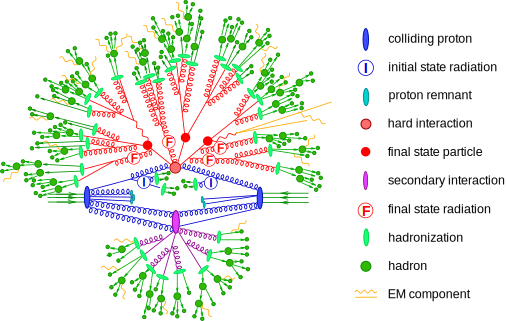
\includegraphics[scale=0.75]{figures/technique/shower.pdf}
}

A brief overview of the event generation and subsequent hadronization programs employed in this thesis is given in the following.

\begin{description}
\item[MadGraph and aMC{@}NLO] fxfx, mlm

\item[Powheg]

\item[Comphep]

\item[Pythia] lund-string model

\item[Herwig] clusters

\end{description}


%##############################################
\section{Top quark reconstruction}
%##############################################

neutrino solution, matching performance

%##############################################
\section{Boosted Decision Trees}
%##############################################
\cite{Hocker:2007ht}

%##############################################
\section{Template-based fitting}
%##############################################

likelihood, barlow-beeston method

%##############################################
\section{Fiducial objects}
%##############################################

dressed leptons, jet clustering, b-tagging

%##############################################
\section{Unfolding}
%##############################################

problems, regularization scheme, correlations, subway plot, alternative FBU
